\begin{frame}
    \frametitle{About Your Fellows}
    \begin{itemize}
        \item Hi there! We are \textcolor{red}{\textbf{Ibrahim}} {and }\textcolor{red}{\textbf{Hammad}}.
        \item We are Associate Students at ITU.
    \end{itemize}
\end{frame}

\section{\textbf{Articulation Points}}

\begin{frame}
    \frametitle{\textbf{Articulation Points}}
        \item\textbf{{Definition:}}
       \vspace{0.3cm}
        \begin{itemize}
            \item Articulation point is a node which if removed increase the number of connected components.
        \end{itemize}
\end{frame}
\begin{frame}
    \frametitle{\textbf{Articulation Point Example}}

    \begin{center}
        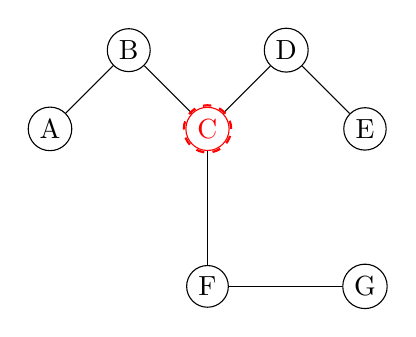
\begin{tikzpicture}[scale=1, every node/.style={draw, circle, inner sep=2pt}]
            % Nodes
            \node (A) at (0, 2) {A};
            \node (B) at (1, 3) {B};
            \node[red] (C) at (2, 2) {C}; % Articulation Point
            \node (D) at (3, 3) {D};
            \node (E) at (4, 2) {E};
            \node (F) at (2, 0) {F};
            \node (G) at (4, 0) {G};

            % Edges
            \draw (A) -- (B);
            \draw (B) -- (C);
            \draw (C) -- (D);
            \draw (D) -- (E);
            \draw (C) -- (F);
            \draw (F) -- (G);

            % Highlight the articulation point
            \draw[red, thick, dashed] (C) circle (0.3);
        \end{tikzpicture}
    \end{center}

    \textbf{Explanation:} The vertex \textcolor{red}{C} is an articulation point because its removal disconnects the graph into three separate components.
\end{frame}

\section{\textbf{Algorithm For Articulation Points}}

\begin{frame}{Articulation Points Algorithm}
    \begin{algorithm}[H]
        \caption{Finding Articulation Points}
        \begin{algorithmic}[1]
            \For{each $x \in V$}
                \State $flag \gets \text{False}$
                \State $t \gets 1$
            \EndFor
            \For{each $v \in N(x)$}
                \If{$v$ is unvisited}
                    \State \textbf{DFS}($v$)
                \EndIf
                 \If{$flag = \text{True}$}
                \State $v$ is an \textbf{Articulation Point (ARTP)}
            \EndIf
            \State $flag \gets \text{True}$
            \EndFor
        \end{algorithmic}
    \end{algorithm}
\end{frame}

\section{\textbf{Depth-First Search Algorithm For Articulation Points}}

\begin{frame}{DFS Algorithm}
    \begin{algorithm}[H]
        \caption{DFS($v$)}
        \begin{algorithmic}[1]
            \State $v.d = t, v.l = t, t \gets t + 1$
            \State $v.visited \gets \text{True}$
            \For{each $u \in N(v)$}
                \If{$u$ is unvisited}
                    \State \textbf{DFS}($u$)
                \EndIf
                \If{$u.d < v.d$ and $u \neq v.\pi$}
                    \State $v.l \gets \min(u.d, v.l)$
                \EndIf
                \If{$u \neq v.\pi$}
                    \State $v.l \gets \min(v.l, u.l)$ \state \textcolor{red}{checking if their is a path to ancestors via child} 
                \EndIf
                \If{$u.l > v.d$}
                    \State $v$ is an \textbf{ARTP}
                \EndIf
            \EndFor
        \end{algorithmic}
    \end{algorithm}
\end{frame}


\begin{frame}
    \frametitle{Complexity}
    \begin{itemize}
        \item Runtime complexity of this algorithm is \textbf{\textcolor{red}{\(\Theta(|V| + |E|)\)}}.
    \end{itemize}
\end{frame}


\section{\textbf{Topological Sort}}

\begin{frame}
    \frametitle{\textbf{Topological Sort}}
    \item\textbf{{Definition:}}
    \vspace{0.3cm}
        \begin{itemize}
            \item It is linear ordering of graph vertices such that for every directed edge uv from vertex u to vertex v,u comes before v in the ordering.
        \end{itemize}
\end{frame}


\begin{frame}
    \frametitle{\textbf{Topological Sort}}
    \item\textbf{{Conditions:}}
    \vspace{0.3cm}
        \begin{itemize}
            \item Tree: Minimally connected graph (there exist a path between every pair vertices).
            \item Directed Acyclic Graph (DAG)
            \item It checks indegrees and outdegrees
        \end{itemize}
\end{frame}

\begin{frame}
     \frametitle{\textbf{Topological Sort}}
     \item\textbf{{Example:}}
     \vspace{0.3cm}
        \begin{itemize}
             \item{\textbf{Task Scheduler}}
             \begin{itemize}
                    \item A Task Scheduler is a system that manages the execution order of tasks while considering dependencies. This is a perfect real-world application of Topological Sorting, which is used in Directed Acyclic Graphs (DAGs) to order tasks such that each task appears before any tasks that depend on it.
                \end{itemize}
        \end{itemize}
\end{frame}

\begin{frame}
    \frametitle{\textbf{How Topological Sorting Works in a Task Scheduler}}
    \begin{itemize}
        \item \textbf{Tasks as Graph Nodes:}
        \begin{itemize}
            \item Each task is represented as a \textbf{node} in a directed graph.
        \end{itemize}
        \vspace{0.3cm}
        \item \textbf{Dependencies as Directed Edges:}
        \begin{itemize}
            \item A directed edge \( A \rightarrow B \) means \textbf{task A must be completed before task B}.
        \end{itemize}
    \end{itemize}
    \begin{itemize}
        \item Check if in-degree is zero. If it is remove it and put it in the list.
        \end{itemize}
\end{frame}

\begin{frame}
    \frametitle{\textbf{Task Dependency Graph (Topological Sorting)}}
    \centering
    \resizebox{0.6\textwidth}{!}{ % Further reduced size
        \begin{tikzpicture}[
            node distance=0.8cm and 1.5cm, % Reduced spacing
            every node/.style={draw, circle, minimum size=0.7cm, font=\small},
            every path/.style={thick, ->}
        ]

        % Define Nodes
        \node (F) {F};
        \node (A) [below left=of F] {A};
        \node (B) [below right=of F] {B};
        \node (D) [below=of B] {D};
        \node (C) [below=of D] {C};
        \node (E) [right=of C] {E};

        % Define Edges (Dependencies)
        \path (F) edge (A);
        \path (F) edge (B);
        \path (A) edge (D);
        \path (B) edge (D);
        \path (D) edge (C);

    \end{tikzpicture}
    }

    \vspace{0.3cm}
    \textbf{Valid Execution Order:} \textcolor{red}{F → A → B → D → C → E}
\end{frame}



\begin{frame}{Topological Sorting Algorithm (1/2)}
    \footnotesize
    \begin{algorithm}[H]
        \caption{Topological Sorting (TS)}
        \begin{algorithmic}[1]
            \State Given a directed graph $G = (V, E)$
            \State Compute in-degrees of all vertices
            \State Initialize an empty queue $W \gets [\ ]$
            \For{each $u \in V$}
                \If{$d(u) = 0$}
                    \State Add $u$ to $W$
                \EndIf
            \EndFor
            
        \end{algorithmic}
    \end{algorithm}
\end{frame}


\begin{frame}{Topological Sorting Algorithm (2/2)}
    \footnotesize
    \begin{algorithm}[H]
        \caption{Topological Sorting (TS) - Continued}
        \begin{algorithmic}[1]
            \While{$W$ is not empty}
                \State Remove a vertex $u$ from $W$
                \For{each outgoing edge $(u, v)$}
                    \State Remove edge $(u, v)$ from $G$
                    \State Decrease in-degree of $v$
                    \If{$d(v) = 0$}
                        \State Add $v$ to $W$
                    \EndIf
                \EndFor
            %\textbf{end while}
            \EndWhile
        \end{algorithmic}
    \end{algorithm}
\end{frame}


\begin{frame}
     \frametitle{\textbf{Topological Sort(Home Work)}}
      \begin{itemize}
        \item Prove this Topological Sort in Linear time \textbf{\textcolor{red}{\(O(V + E)\)}}.
    \end{itemize}
\end{frame}